\documentclass[notes, handout]{beamer}
%\documentclass[notes]{beamer}

\usepackage{amsmath}
\usepackage{amssymb}
\usepackage{algorithmic}
\usepackage{subfigure}
\usepackage{multirow}
\usepackage{graphicx}

\graphicspath{{figures/}}

\usetheme{CambridgeUS}
\usecolortheme{seagull}

\beamertemplatenavigationsymbolsempty

\title[LSD Software]{Software and computing environment}
\author{Mathieu Gagnon}
\institute[LSD, U. Laval]{LSD \\ Laval University}
\date{2010-02-24}

\begin{document}

\frame{\titlepage}

\section*{Plan}

\begin{frame}
	\frametitle{Plan}
	\begin{itemize}
		\item SCHNAPS
		\item LSD Input GUI
		\item LSD Output GUI
		\item Computing environment
	\end{itemize}
\end{frame}

\section*{SCHNAPS}

\begin{frame}
	\frametitle{SCHNAPS : a public health generic simulator}
	\begin{itemize}
		\item SynCHroNous Agent and Population-based Simulator
		\item Coded in C++
		\item Command line-driven (no graphical front-end)
		\item Extensible and Versatile
	\end{itemize}
\end{frame}

\begin{frame}
	\frametitle{SCHNAPS: Agent and Population-based}
	\begin{itemize}
		\item<1-> System PoV:
			\begin{itemize}
				\item Agent-based: Explicitly defined entities.
				\item Population-based: Homogeneous group of agents.
			\end{itemize}
		\item<2-> Public Health PoV:
			\begin{itemize}
				\item Agent: virtual individuals.
				\item Population: all virtual individuals in the simulator at a given time.
			\end{itemize}
	\end{itemize}
\end{frame}

\begin{frame}
	\frametitle{SCHNAPS: Virtual individuals}
	\begin{itemize}
		\item<1-> Virtual individuals are made of variables
		\item<2-> Each virtual individual owns its set of variables
		\item<3-> The environment, a meta-individual, holds variables common to all virtual individuals
	\end{itemize}
\end{frame}

\begin{frame}
	\frametitle{SCHNAPS: Time-driven}
	\begin{itemize}
		\item Events are triggered at each clock step
		\item Time is an independant variable
	\end{itemize}
\end{frame}

\begin{frame}
	\frametitle{SCHNAPS: Framework}
	\includegraphics[width=\textwidth]{framework}
\end{frame}

\begin{frame}
	\frametitle{Trees}
	\begin{itemize}
		\item<1-> Decisions trees are built with primitives (nodes)
		\item<2-> Base primitives have been created at the beginning
			\begin{itemize}
				\item Math
				\item Control (Branching)
				\item Data
			\end{itemize}
		\item<3-> Specialized primitives have been added
			\begin{itemize}
				\item Event
				\item Test
				\item Treatment
			\end{itemize}
		\item<4-> Decision tree has to be separated in mutiple subtrees, called processes
	\end{itemize}
\end{frame}

\begin{frame}
	\frametitle{Processes}
	\begin{itemize}
		\item<1-> Scenario: First process to be applied
		\item<2-> Called: Processes can be called for immediate execution.
		\item<3-> Pushed: Processes can be pushed for delayed execution.
		\item<4-> Observers: Processes called every time the clock value changes
	\end{itemize}
\end{frame}

\begin{frame}
	\frametitle{Learning module}
	\begin{itemize}
		\item Learning module is a plugin
		\item It can optimize cost/effectiveness:
		\begin{itemize}
			\item in the right combination of tests/treatments to use
			\item in the right groups of the population to target
		\end{itemize}
	\end{itemize}
\end{frame}

\section*{LSD Input GUI}
\begin{frame}
	\frametitle{Input GUI}
	\begin{itemize}
		\item Simulations are defined in configuration files
		\item File are written in XML(eXtensible Markup Language)
		\item Input GUI aims at : 
		\begin{itemize}
			\item Presenting the XML files in a user-friendly way
			\item Giving tools to start new XML files
			\item Giving tools to edit existing XML files
		\end{itemize} 
	\end{itemize}
\end{frame}

\section*{LSD Output GUI}
\begin{frame}
	\frametitle{Output GUI}
	\begin{itemize}
		\item Results outputed by SCHNAPS are hard to understand for non-programers
		\item They are stored on a server
		\item Output GUI aims at : 
		\begin{itemize}
			\item{Retrieving the output files from the server}
			\item{Presenting the output files in a user-friendly way}
			\item{Giving tools to analyze the results}
		\end{itemize} 
	\end{itemize}
\end{frame}

\section*{Computing environment}
\begin{frame}
	\frametitle{Computers, softwares and communications}
	\begin{itemize}
	\item LSD Group:
		\begin{itemize}
			\item Owns a server to store simulation results
			\item Has access to CLUMEQ's supercomputer, Colosse
		\end{itemize}
	\item Computing environment aims at:
		\begin{itemize}
			\item Giving tools to easily create configuration files
			\item Automatically sending jobs to SCHNAPS, hosted on Colosse
			\item Automatically sending simulation results to the LSD server
			\item Giving tools to easily retrieve and analyze the results
		\end{itemize}
	\end{itemize}
\end{frame}

\begin{frame}
	\frametitle{Computing Environment : Framework}
	\begin{center}
	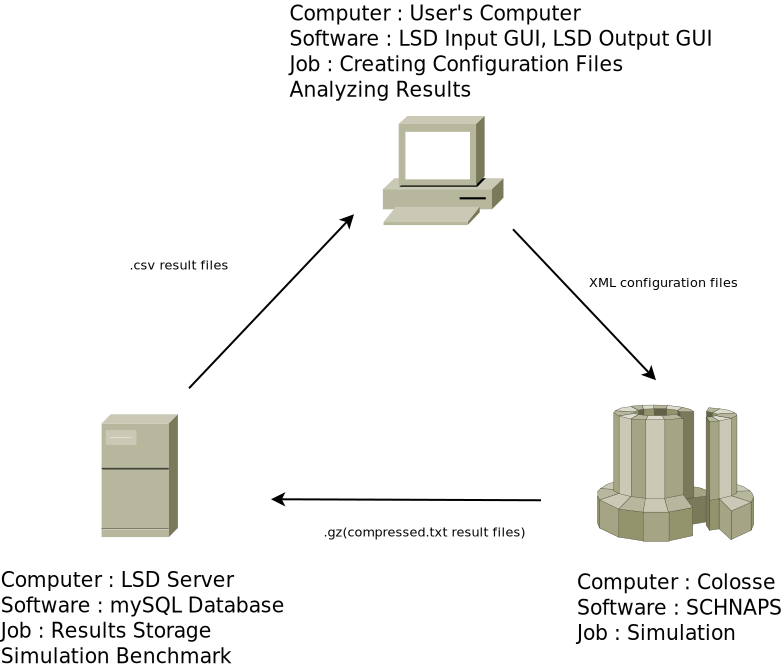
\includegraphics[scale=0.18]{Diagram1}
	\end{center}
\end{frame}

\end{document}
